\documentclass{article}
\usepackage{amsmath}
\usepackage{amsfonts}
\usepackage{graphicx}
\usepackage{parskip}
\setlength{\parindent}{0pt}
\setlength{\parskip}{5pt}
\title{HW 5}
\author{Max Horowitz-Gelb}
\date{2/20/17}

\begin{document}
\maketitle
\section*{Q1}
For a two state THMC with transitions probabilities,
\[
\begin{bmatrix}
1-a & a\\
b & 1-b
\end{bmatrix}
\]
Our stationary distribution is simply,
\[
[\frac{b}{a+b}, \frac{a}{a+b}] = [\frac{1}{7}, \frac{6}{7}]
\]

\section*{Q2}
We must solve for
\[
\pi p = p
\]
This gives us the set of equations
\[
\pi_1 = \pi_1
\]
\[
0.4\pi_2 + 0.1\pi_3 = \pi_2
\]
\[
0.6\pi_2 + 0.9\pi_3 = \pi_3
\]
\[
\pi_1 + \pi_2 + \pi_3 = 1
\]
\[
\pi_1, \pi_1, \pi_3 \in [0,1]
\]
Solving for these equations you get that $\pi_1$ is free $\pi_2 = (1/7)(1-\pi_1) $and $\pi_3 = (6/7)(1-\pi_1)$.
So the the staitionary distributions are
\[
[\pi_1, (1/7)(1-\pi_1), (6/7)(1-\pi_1)]  \text{ for any } \pi_1 \in [0,1]
\] 

\section*{Q3}
If
\[
v = vp
\]
then,
\[
(-1/10)v = -(1/10)vp
\]
therefore
\[
[1/10,2/10,3/10,4/10]
\]
is also a stationary measure, and since its elements sum to 1 and are positive then it is a stationary distribution.



\section*{Q4}

\subsection*{a}
For a single step it is simply,
\begin{tabular}{|l|l|l|l|l|}
\hline
 & RR & RS & SR & SS \\ \hline
RR & 0.6 & 0.4 & 0 & 0\\ \hline
RS & 0& 0 &0.6 & 0.4\\ \hline
SR & 0.6 & 0.4 & 0 & 0\\ \hline
SS & 0 &0 & 0.3 & 0.7 \\ \hline
\end{tabular}
\subsection*{b}
For two steps we must calculate two transitions which gives us


\begin{tabular}{| l | l | l | l |l|}
	\hline
     & RR & RS & SR & SS \\ \hline
    RR & 0.6 * 0.6 & 0.6 * 0.4 & 0.4 * 0.6 & 0.4 * 0.4 \\ \hline
    RS & 0.6* 0.6 & 0.6 * 0.4 & 0.4* 0.3 & 0.4 * 0.7 \\ \hline
    SR & 0.6 * 0.6 & 0.6 * 0.4 & 0.4 * 0.6 & 0.4 * 0.4 \\ \hline
    SS & 0.3*0.6 & 0.3 * 0.4 & 0.7 * 0.3 & 0.7 * 0.7 \\ \hline 
\end{tabular}

which is,
\begin{tabular}{| l | l | l | l |l|}
	\hline
     & RR & RS & SR & SS \\ \hline
    RR & 0.36 & 0.24 & 0.24 & 0.16 \\ \hline
    RS & 0.36 & 0.24 & 0.12 & 0.28 \\ \hline
    SR & 0.36 & 0.24 & 0.24 & 0.16 \\ \hline
    SS & 0.18 & 0.12 & 0.21 & 0.49 \\ \hline 
\end{tabular}

\subsection*{c}
The probability it will rain on Wednesday given it did not rain on Sunday or Monday is equal to 
\[
P(SS \rightarrow RR ) + P(SS \rightarrow SR) = 0.18 + 21 = 0.39
\]


\section*{Q5}
Let our set of states be ${1,2}$ with tranition probability matrix
$
\begin{bmatrix}
0 & 1 \\
0 & 1 \\
\end{bmatrix}
$. Then state 1 is transient and state 2 is recurrent. Clearly state 1 is transient since with probability 1 it will transition from state 1 to 2, and there is no way to transition back to 1. Clearly state 2 is recurrent since it will always transition back to itself with proability 1. 

\section*{Q6}
For a state set of {1,2,3,4,5,6} we define the transition probabilities graphically,
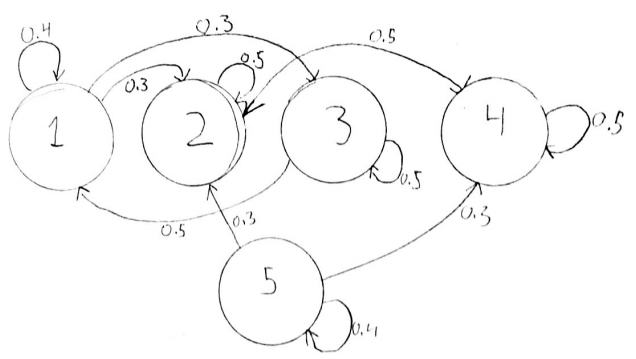
\includegraphics[scale=0.5]{transition}

State 1 is clearly transient since it only has an outgoing edge. 

States 2 and 3 both have period 2 since both will travel to the other and then travel back to theirselves with probability 1, which takes two transitions.

States 4,5 and 6 all have period 3, since all of them with probability 1 will travel once to each of the other nodes before returning to theirselves which takes three transitions.

\section*{Q7}
State -2 starts in the triangle, so it will return to itself after at least once going through the triangle and some number of times through the square so,
$I_{-2} = \{3a + 4b : a \in \mathbb{N} , b \in \mathbb{N} \cup \{0\} \}$

3 and 7 exist in $I_{-2}$ and the gcd of these is 1 so state -2 has period 1.

State 2 starts in the square, so it will return to itself after at least once going through the square and some number of times throught the triangle so, 
$I_{2} = \{3a + 4b : a \in \mathbb{N} \cup \{0\} , b \in \mathbb{N}\}$
4 and 7 are in $I_2$ and they have a gcd of 1 so state 2 has a period of 1.



\end{document}